\documentclass[letterpaper]{article}

\usepackage{geometry}
\newgeometry{vmargin={25mm}, hmargin={30mm,30mm}}

\setcounter{secnumdepth}{0}

\usepackage{noto}

\usepackage{amsmath}
\usepackage{listings}
\usepackage{xcolor}
\usepackage{multirow}
\usepackage{float,graphicx}
\usepackage{subcaption}
\usepackage[breaklinks=true]{hyperref}
\appto\UrlBreaks{\do\-}

\usepackage{mdframed}
\newenvironment{modeloutput}[1]{%
	\begin{mdframed}[backgroundcolor=gray!8, linecolor=gray!60, linewidth=0.8pt,
		innerleftmargin=8pt, innerrightmargin=8pt, innertopmargin=6pt, innerbottommargin=6pt]%
	\small\ttfamily\raggedright
}{%
	\end{mdframed}%
}

\lstset{
	basicstyle=\small\ttfamily,
	tabsize=4,
	frame=single,
	breaklines,
	postbreak=\mbox{\textcolor{red}{$\hookrightarrow$}\space},
	showstringspaces=false,
}

\begin{document}
\title{Assignment 1: Basics}

\author{Ethan Chung\\
    {\tt\small University of Hawaii}\\
    {\tt\small ECE 405: Intro to Large-Scale AI Systems}\\
    {\tt\small [redacted]@hawaii.edu}}

\maketitle

\tableofcontents

\newpage

\section{Byte-Pair Encoding (BPE) Tokenizer}

\subsection{Problem (unicode1): Understanding Unicode (1 point)}

\begin{itemize}
	\item[(a)] What Unicode character does \texttt{chr(0)} return?

	\texttt{chr(0)} returns \texttt{\textbackslash x00}, which is the Unicode character U+0000 or the null byte.

	\item[(b)] How does this character's string representation (\texttt{\_\_repr\_\_()}) differ from its printed representation?

	\texttt{chr(0).\_\_repr\_\_()} shows the escaped value with \texttt{"'\textbackslash x00'"}, while the printed representation is the raw character output, which is invisible and appears to show nothing.

	\item[(c)] What happens when this character occurs in text?

	\begin{lstlisting}[language=Python]
		>>> chr(0)
		'\x00'
		>>> print(chr(0))

		>>> "this is a test" + chr(0) + "string"
		'this is a test\x00string'
		>>> print("this is a test" + chr(0) + "string")
		this is a teststring
		>>> x = "a" + chr(0); print(x); x[1];
		a
		'\x00'
	\end{lstlisting}
\end{itemize}

The string is evaluated as a null byte \verb|\x00|, which prints nothing (although it does still exist in the string as proven by the fifth eval).

\subsection{Problem (unicode2): Unicode Encodings (3 points)}

\begin{itemize}
	\item[(a)] What are some reasons to prefer training our tokenizer on UTF-8 encoded bytes, rather than UTF-16 or UTF-32?

UTF-8 encoded bytes range from [0,255], whereas the UTF-16 and UTF-32 would range from [0,65535] and [0,4294967295], respectively. Using either of these would negate our goal of trying to compress the sequence of integers into something manageable for token vocab to stay small.

	\item[(b)] Consider the following (incorrect) function, which is intended to decode a UTF-8 byte string into a Unicode string. Why is this function incorrect? Provide an example of an input byte string that yields incorrect results.

If I use "¥" (which is \texttt{b'\textbackslash xC2\textbackslash xA5'}) for the byte string, it results in the following error:

\begin{lstlisting}[language=Python]
def decode_utf8_bytes_to_str_wrong(bytestring: bytes):
	return "".join([bytes([b]).decode("utf-8") for b in bytestring])

>>> decode_utf8_bytes_to_str_wrong("hello".encode("utf-8"))
'hello'

>>> decode_utf8_bytes_to_str_wrong("¥".encode("utf-8"))
UnicodeDecodeError: 'utf-8' codec can't decode byte 0xc2 in position 0: unexpected end of data
\end{lstlisting}

Unicode has variable-length multi-byte sequences and for symbols outside of the standard ASCII set, it will use multiple bytes to represent a single character, whereas this implementation assumes all characters = 1 byte.

	\item[(c)] Give a two byte sequence that does not decode to any Unicode character(s).

\begin{lstlisting}[language=Python]
>>> "ẜ".encode("utf-8")
b'\xe1\xba\x9c'

>>> b'\xe1\xba'.decode("utf-8")
UnicodeDecodeError: 'utf-8' codec can't decode bytes in position 0-1: unexpected end of data
\end{lstlisting}

\verb|\xe1| describes that there should be three bytes present in the string to form the character, but only two were provided in the decode, thus it errors due to a mismatch in the sequence length.

\end{itemize}

\subsection{Problem (train\_bpe): BPE Tokenizer Training (15 points)}

\textit{Implemented in  \href{https://github.com/echung32/ece405-assignment1-basics/blob/main/cs336_basics/train_bpe.py}{cs336\_basics/train\_bpe.py}}

\subsection{Problem (train\_bpe\_tinystories): BPE Training on TinyStories (2 points)}

\begin{itemize}
	\item[(a)] Train a byte-level BPE tokenizer on the TinyStories dataset, using a maximum vocabulary size
	of 10,000. How many hours and memory did training take? What is the longest token in the vocabulary? Does it make sense?

	Training took a total of 99.54 seconds, utilizing peak memory usage of 118.01 MB, and the longest token in the vocabulary was found to be 15 bytes long for \texttt{" accomplishment"}. This does make sense, as it is likely the result of merging the subwords of \texttt{" accomplish"} and \texttt{"ment"} together.

	\item[(b)] What part of the tokenizer training process takes the most time?

	Breaking down the total time, the longest ranked from top to bottom are:

\begin{center}
\begin{tabular}{lr}
\hline
\textbf{Step} & \textbf{Time (s)} \\
\hline
Pre-tokenization & 55.95 \\
Merge loop (total) & 36.27 \\
Merge updates (total) & 2.90 \\
Pair count initialization & 0.31 \\
Vocabulary initialization & 0.00 \\
\hline
\end{tabular}
\end{center}

	The pre-tokenization step dominates, taking 55.95s out of 99.54s total. This makes sense as it involves scanning the entire dataset to split text into initial tokens before any merges can begin.
\end{itemize}

\textit{Implemented in  \href{https://github.com/echung32/ece405-assignment1-basics/blob/main/scripts/train_bpe_dataset.py}{scripts/train\_bpe\_dataset.py}}

\subsection{Problem (train\_bpe\_expts\_owt): BPE Training on OpenWebText (2 points)}

\begin{itemize}
	\item[(a)] Train a byte-level BPE tokenizer on the OpenWebText dataset, using a maximum vocabulary
	size of 32,000. What is the longest token in the vocabulary? Does it make sense?

	The longest token consisted of 64 bytes and is the string \texttt{ÃÂÃÂÃÂÃÂÃÂÃÂÃÂÃÂÃÂÃÂÃÂÃÂ\allowbreak ÃÂÃÂÃÂÃÂ} (the characters \texttt{Ã} (U+00C3) and \texttt{Â} (U+00C2) repeated 16 times), which are present in the original dataset and is likely caused by \textit{mojibake} artifacts from double-encoding UTF-8 text as Latin-1.

	\item[(b)] Compare and contrast the tokenizer that you get training on TinyStories versus OpenWebText.

	The TinyStories tokenizer learns simpler vocabulary tokens from children's stories which contain simplistic phrases, while the OpenWebText tokenizer contains a more broad and diverse vocabulary from the internet. The OWT tokenizer also captures more domain-specific subwords, like technical terms, punctuation patterns, URLs, etc.

\end{itemize}

\textit{Implemented in  \href{https://github.com/echung32/ece405-assignment1-basics/blob/main/scripts/train_bpe_dataset.py}{scripts/train\_bpe\_dataset.py}}

\subsection{Problem (tokenizer): Implementing the tokenizer (15 points)}

\textit{Implemented in \href{https://github.com/echung32/ece405-assignment1-basics/blob/main/cs336_basics/tokenizer.py}{cs336\_basics/tokenizer.py}}

\subsection{Problem (tokenizer\_experiments): Experiments with tokenizers (4 points)}

\begin{itemize}
	\item[(a)] Sample 10 documents from TinyStories and OpenWebText. Using your previously-trained TinyStories and OpenWebText tokenizers (10K and 32K vocabulary size, respectively), encode these sampled documents into integer IDs. What is each tokenizer’s compression ratio (bytes/token)?

\begin{center}
\begin{tabular}{lrrr}
\hline
\textbf{Dataset} & \textbf{Total Bytes} & \textbf{Total Tokens} & \textbf{Compression Ratio} \\
\hline
TinyStories & 7,513 & 1,812 & 4.146 bytes/token \\
OpenWebText & 38,175 & 8,653 & 4.412 bytes/token\\
\hline
\end{tabular}
\end{center}

	The OpenWebText tokenizer achieves a 6.4\% better compression ratio than the TinyStories tokenizer on their respective datasets, which is expected given its larger vocabulary size (32K vs.\ 10K) allowing it to encode more text per token.

	\item[(b)] What happens if you tokenize your OpenWebText sample with the TinyStories tokenizer? Compare the compression ratio.

\begin{center}
\begin{tabular}{lrrr}
\hline
\textbf{Tokenizer} & \textbf{Total Bytes} & \textbf{Total Tokens} & \textbf{Compression Ratio} \\
\hline
OWT tokenizer on OWT & 38,175 & 8,653 & 4.412 bytes/token \\
TS tokenizer on OWT & 36,380 & 11,653 & 3.122 bytes/token \\
\hline
\end{tabular}
\end{center}

	Applying the TinyStories tokenizer to the OpenWebText sample yields a 29.2\% worse compression ratio (3.122 vs.\ 4.412 bytes/token). This is expected, as the TinyStories tokenizer has not learned the vocabulary of more diverse web text, so it falls back to shorter and less efficient token merges.

	\item[(c)] Estimate the throughput of your tokenizer (e.g., in bytes/second). How long would it take to tokenize the Pile dataset (825GB of text)?

\begin{center}
\begin{tabular}{lr}
\hline
\textbf{Tokenizer} & \textbf{Throughput} \\
\hline
TinyStories & 1,466,294 bytes/s (1.47 MB/s) \\
OpenWebText & 1,242,250 bytes/s (1.24 MB/s) \\
\hline
\end{tabular}
\end{center}

	Throughput was measured qualitatively by averaging the encoding over 5 runs. At 1.47 MB/s, tokenizing the 825 GB Pile dataset would take approximately 167.8 hours using the TinyStories tokenizer; at 1.24 MB/s with the OpenWebText tokenizer, approximately 198.1 hours. The OWT tokenizer is slightly slower, likely because its larger vocabulary (32K) requires searching a larger merge table on each step.

	\item[(d)] Using your TinyStories and OpenWebText tokenizers, encode the respective training and devel-
	opment datasets into a sequence of integer token IDs. We recommend serializing the token IDs as a NumPy array of datatype uint16. Why is uint16 an appropriate choice?

	\texttt{uint16} stores values in the range $[0, 65535]$, which comfortably covers both vocabulary sizes (10K and 32K) and only costs 2 bytes per token. Using \texttt{uint8} ($[0, 255]$) would be too small to index either vocabulary, while \texttt{uint32} would double the storage cost to 4 bytes per token unnecessarily.

\end{itemize}

\textit{Implemented in  \href{https://github.com/echung32/ece405-assignment1-basics/blob/main/scripts/tokenizer_experiments.py}{scripts/tokenizer\_experiments.py}}

\section{Transformer Language Model Architecture}

\subsection{Problem (linear): Implementing the linear module (1 point)}

\textit{Implemented in  \href{https://github.com/echung32/ece405-assignment1-basics/blob/main/cs336_basics/module/linear.py}{cs336\_basics/module/linear.py}}

\subsection{Problem (embedding): Implement the embedding module (1 point)}

\textit{Implemented in  \href{https://github.com/echung32/ece405-assignment1-basics/blob/main/cs336_basics/module/embedding.py}{cs336\_basics/module/embedding.py}}

\subsection{Problem (rmsnorm): Root Mean Square Layer Normalization (1 point)}

\textit{Implemented in  \href{https://github.com/echung32/ece405-assignment1-basics/blob/main/cs336_basics/module/rmsnorm.py}{cs336\_basics/module/rmsnorm.py}}

\subsection{Problem (positionwise\_feedforward): Implement the position-wise feed-forward network (2 points)}

\textit{Implemented in  \href{https://github.com/echung32/ece405-assignment1-basics/blob/main/cs336_basics/module/swiglu.py}{cs336\_basics/module/swiglu.py}}

\subsection{Problem (rope): Implement RoPE (2 points)}

\textit{Implemented in  \href{https://github.com/echung32/ece405-assignment1-basics/blob/main/cs336_basics/module/rope.py}{cs336\_basics/module/rope.py}}

\subsection{Problem (softmax): Implement softmax (1 point)}

\textit{Implemented in  \href{https://github.com/echung32/ece405-assignment1-basics/blob/main/cs336_basics/softmax.py}{cs336\_basics/softmax.py}}

\subsection{Problem (scaled\_dot\_product\_attention): Implement scaled dot-product attention (5 points)}

\textit{Implemented in  \href{https://github.com/echung32/ece405-assignment1-basics/blob/main/cs336_basics/attention.py}{cs336\_basics/attention.py}}

\subsection{Problem (multihead\_self\_attention): Implement causal multi-head self-attention (5 points)}

\textit{Implemented in \href{https://github.com/echung32/ece405-assignment1-basics/blob/main/cs336_basics/module/multihead_attention.py}{cs336\_basics/module/multihead\_attention.py}}

\subsection{Problem (transformer\_block): Implement the Transformer block (3 points)}

\textit{Implemented in  \href{https://github.com/echung32/ece405-assignment1-basics/blob/main/cs336_basics/module/transformer_block.py}{cs336\_basics/module/transformer\_block.py}}

\subsection{Problem (transformer\_lm): Implementing the Transformer LM (3 points)}

\textit{Implemented in  \href{https://github.com/echung32/ece405-assignment1-basics/blob/main/cs336_basics/transformer_lm.py}{cs336\_basics/transformer\_lm.py}}

\subsection{Problem (transformer\_accounting): Transformer LM resource accounting (5 points)}

\begin{itemize}
	\item[(a)] Consider GPT-2 XL, which has the following configuration:

	\begin{center}
	\begin{tabular}{lll}
		\texttt{vocab\_size} & 50,257 & ($V$) \\
		\texttt{context\_length} & 1,024 & ($T$) \\
		\texttt{num\_layers} & 48 & ($L$) \\
		\texttt{d\_model} & 1,600 & ($d$) \\
		\texttt{num\_heads} & 25 & ($H$,\ $d_k = d/H = 64$) \\
		\texttt{d\_ff} & 6,400 & ($d_\text{ff}$) \\
	\end{tabular}
	\end{center}

	Suppose we constructed our model using this configuration. How many trainable parameters would our model have? Assuming each parameter is represented using single-precision floating point, how much memory is required to just load this model?

	\begin{center}
	\begin{tabular}{lr}
	\hline
	\textbf{Component} & \textbf{Parameters} \\
	\hline
	Token embedding $(V \times d)$ & $50{,}257 \times 1{,}600 = 80{,}411{,}200$ \\
	\hline
	\multicolumn{2}{l}{\textit{Per transformer block ($\times L = 48$):}} \\
	\quad $q\_\text{proj}$, $k\_\text{proj}$, $v\_\text{proj}$, $\text{output\_proj}$ (each $d\times d$) & $4 \times d^2 = 4 \times 2{,}560{,}000 = 10{,}240{,}000$ \\
	\quad $w_1$, $w_3$, $w_2$ (each $d_\text{ff}\times d$ or $d\times d_\text{ff}$) & $3 \times d\,d_\text{ff} = 3 \times 10{,}240{,}000 = 30{,}720{,}000$ \\
	\quad RMSNorm $\times 2$ (each weight shape $(d,)$) & $2 \times d = 2 \times 1{,}600 = 3{,}200$ \\
	\quad \textit{Per block subtotal} & $40{,}963{,}200$ \\
	\hline
	Final RMSNorm $(d,)$ & $1{,}600$ \\
	LM head $(V \times d$) & $80{,}411{,}200$ \\
	\hline
	\textbf{Total} & $\mathbf{2{,}127{,}057{,}600}$ \\
	\hline
	\end{tabular}
	\end{center}

	Deriving the formula from the per-component breakdown:
	\[
		P = \underbrace{Vd}_{\text{embedding}} + L\underbrace{(4d^2 + 3d\,d_\text{ff} + 2d)}_{\text{per block}} + \underbrace{d}_{\text{final norm}} + \underbrace{Vd}_{\text{LM head}}
		= 2{,}127{,}057{,}600 \approx 2.13\text{ billion parameters}
	\]
	At 4 bytes per float32 parameter, loading the model requires $4P = 8{,}508{,}230{,}400\text{ bytes} \approx 8.51\text{ GB}$.

	\item[(b)] Identify the matrix multiplies required to complete a forward pass of our GPT-2 XL-shaped model. How many FLOPs do these matrix multiplies require in total? Assume that our input sequence has \texttt{context\_length} tokens.

	\textbf{Per transformer block ($\times L$ blocks):}

	\begin{table}[H]
	\centering
	\begin{tabular}{llll}
	\hline
	\textbf{Operation} & \textbf{Description} & \textbf{Dimensions} & \textbf{FLOPs per block} \\
	\hline
	Q projection & Input $\to$ queries via $W_Q$ & $(T,d)\times(d,d)$ & $2Td^2 = 5.24\times10^9$ \\
	K projection & Input $\to$ keys via $W_K$ & $(T,d)\times(d,d)$ & $2Td^2 = 5.24\times10^9$ \\
	V projection & Input $\to$ values via $W_V$ & $(T,d)\times(d,d)$ & $2Td^2 = 5.24\times10^9$ \\
	$QK^\top$ (scores) & $\sum_{h=1}^{H} (T,d_k)\times(d_k,T)$ & $H\times(T,d_k)\times(d_k,T)$ & $2T^2d = 3.36\times10^9$ \\
	Attn$\times V$ (output) & $\sum_{h=1}^{H} (T,T)\times(T,d_k)$ & $H\times(T,T)\times(T,d_k)$ & $2T^2d = 3.36\times10^9$ \\
	Output projection & Concat heads $\to$ $W_O$ & $(T,d)\times(d,d)$ & $2Td^2 = 5.24\times10^9$ \\
	SwiGLU $W_1$ (gate branch) & Input $\to$ $d_\text{ff}$ via $W_1$ & $(T,d)\times(d,d_\text{ff})$ & $2Td\,d_\text{ff} = 20.97\times10^9$ \\
	SwiGLU $W_3$ (linear branch) & Input $\to$ $d_\text{ff}$ via $W_3$ & $(T,d)\times(d,d_\text{ff})$ & $2Td\,d_\text{ff} = 20.97\times10^9$ \\
	SwiGLU $W_2$ (output) & $d_\text{ff}\to$ output via $W_2$ & $(T,d_\text{ff})\times(d_\text{ff},d)$ & $2Td_\text{ff}\,d = 20.97\times10^9$ \\
	\hline
	\end{tabular}
	\end{table}

	Additionally, adding the single LM head which takes hidden state $\to$ vocab logits, of shape $(T,d)\times(d,V)$, the FLOPs per block is $2TdV = 1.65\times10^{11}$, and thus the total is:

	\[
		\text{Total} = L(8Td^2 + 4T^2d + 6Td\,d_\text{ff}) + 2TdV \approx 4.513\times10^{12}\text{ FLOPs}
	\]

	\item[(c)] Based on your analysis above, which parts of the model require the most FLOPs?

	The SwiGLU feed-forward network consumes 66.9\% of total FLOPs (3,019.8B of 4,513B), since it requires three $(T,d)\times(d,d_\text{ff})$ matrix multiplies per layer. % The four attention projections (Q, K, V, O) account for 22.3\% (1,006.8B), while the quadratic attention score and value-weighting products ($QK^\top$ and Attn$\times V$) account for only 7.1\% (322.2B). The LM head contributes just 3.7\% (165.0B).

	\item[(d)] Repeat your analysis with GPT-2 small (12 layers, 768 \texttt{d\_model}, 12 heads), GPT-2 medium (24 layers, 1024 \texttt{d\_model}, 16 heads), and GPT-2 large (36 layers, 1280 \texttt{d\_model}, 20 heads). As the model size increases, which parts of the Transformer LM take up proportionally more or less of the total FLOPs?

	\begin{center}
	\begin{tabular}{lrrrr}
	\hline
	\textbf{Component} & \textbf{Small} & \textbf{Medium} & \textbf{Large} & \textbf{XL} \\
	\hline
	Total FLOPs & 0.35 TF & 1.03 TF & 2.26 TF & 4.51 TF \\
	\hline
	Attn projections (Q/K/V/O) & 16.5\% & 20.0\% & 21.5\% & 22.3\% \\
	Attn core ($QK^\top$ + AV) & 11.1\% & 10.0\% & 8.6\% & 7.1\% \\
	FFN (all layers) & 49.8\% & 59.9\% & 64.2\% & 66.9\% \\
	LM head & 22.6\% & 10.2\% & 5.8\% & 3.7\% \\
	\hline
	\end{tabular}
	\end{center}

	As model size increases, the FFN dominates more ($\sim$50\% $\to$ $\sim$67\%), since FFN cost scales as $O(Ld^2 T)$ while the LM head scales only as $O(TdV)$, making the fixed-vocabulary head relatively cheaper as $d$ and $L$ grow. The attention core products $O(LT^2d)$ shrink proportionally because $T$ is fixed while $d$ and $L$ grow, whereas the $O(Ld^2 T)$ attention projections grow in step with the FFN.

	\item[(e)] Take GPT-2 XL and increase the context length to 16,384. How does the total FLOPs for one forward pass change? How do the relative contribution of FLOPs of the model components change?

	Increasing context length from 1,024 to 16,384 increases total FLOPs by approximately 33$\times$ (from 4.51 TFLOPs to $\approx1.50\times10^{14}$ FLOPs $\approx$ 150 TFLOPs), because the attention $QK^\top$ and AV products scale quadratically with $T$. As a result, the attention core ($QK^\top$ + AV) grows from 7.1\% to 55.2\% of total FLOPs, FFN drops from 66.9\% to 32.3\%, and attention projections drop from 22.3\% to 10.8\%.

\end{itemize}

\section{Training a Transformer LM}

\subsection{Problem (cross\_entropy): Implement Cross entropy}

\textit{Implemented in  \href{https://github.com/echung32/ece405-assignment1-basics/blob/main/cs336_basics/cross_entropy.py}{cs336\_basics/cross\_entropy.py}}

\subsection{Problem (learning\_rate\_tuning): Tuning the learning rate (1 point)}

\begin{quote}
	Run the SGD example with three other values for the learning rate: 1e1, 1e2, and 1e3, for just 10 training iterations. What happens with the loss for each of these learning rates? Does it decay faster, slower, or does it diverge (i.e., increase over the course of training)?
\end{quote}

With \texttt{lr=1e1} the loss decays faster than the baseline (\texttt{lr=1}), reaching 3.25 after 10 iterations vs.\ 20.0; with \texttt{lr=1e2} the loss converges extremely rapidly, collapsing to near-zero by iteration 4 ($1.49 \times 10^{-16}$). With \texttt{lr=1e3} the loss diverges from 24.2 to $2.24 \times 10^{18}$ over 10 iterations.

\textit{Implemented in  \href{https://github.com/echung32/ece405-assignment1-basics/blob/main/scripts/sgd_learning_rates.py}{scripts/sgd\_learning\_rates.py}}

\subsection{Problem (adamw): Implement AdamW (2 points)}

\textit{Implemented in  \href{https://github.com/echung32/ece405-assignment1-basics/blob/main/cs336_basics/optimizer/adamw.py}{cs336\_basics/adamw.py}}

\subsection{Problem (adamwAccounting): Resource accounting for training with AdamW (2 points)}

\begin{itemize}
	\item[(a)] How much peak memory does running AdamW require? Decompose your answer based on the memory usage of the parameters, activations, gradients, and optimizer state. Express your answer in terms of the \texttt{batch\_size} and the model hyperparameters (\texttt{vocab\_size}, \texttt{context\_length}, \texttt{num\_layers}, \texttt{d\_model}, \texttt{num\_heads}). Assume \texttt{d\_ff = 4 × d\_model}.

	\textbf{Activations.}

	\begin{table}[H]
	\centering
	\begin{tabular}{llr}
	\hline
	\textbf{Operation} & \textbf{Output shape} & \textbf{Elements} \\
	\hline
	\multicolumn{3}{l}{\textit{Per transformer block ($\times L$):}} \\
	\quad RMSNorm ln1 & $(B,T,d)$ & $BTd$ \\
	\quad Q projection & $(B,T,d)$ & $BTd$ \\
	\quad K projection & $(B,T,d)$ & $BTd$ \\
	\quad V projection & $(B,T,d)$ & $BTd$ \\
	\quad $QK^\top$ scores & $(B,H,T,T)$ & $BHT^2$ \\
	\quad Softmax & $(B,H,T,T)$ & $BHT^2$ \\
	\quad Weighted sum (Attn$\times V$) & $(B,T,d)$ & $BTd$ \\
	\quad Output projection & $(B,T,d)$ & $BTd$ \\
	\quad RMSNorm ln2 & $(B,T,d)$ & $BTd$ \\
	\quad $W_1$ output & $(B,T,d_\text{ff})$ & $4BTd$ \\
	\quad SiLU output & $(B,T,d_\text{ff})$ & $4BTd$ \\
	\quad $W_2$ output & $(B,T,d)$ & $BTd$ \\
	\quad \textit{Per block subtotal} & & $17BTd + 2BHT^2$ \\
	\hline
	\multicolumn{3}{l}{\textit{Outside blocks:}} \\
	\quad Final RMSNorm & $(B,T,d)$ & $BTd$ \\
	\quad LM head & $(B,T,V)$ & $BTV$ \\
	\quad Cross-entropy softmax & $(BT,V)$ & $BTV$ \\
	\hline
	\end{tabular}
	\end{table}
	\[
		A = L(17BTd + 2BHT^2) + BT(d + 2V)
	\]

		\textbf{Parameters.}

	\begin{center}
		\begin{tabular}{lr}
			\hline
			\textbf{Component} & \textbf{Parameter count} \\
			\hline
			Token embedding $(V \times d)$ & $Vd$ \\
			\hline
			\multicolumn{2}{l}{\textit{Per transformer block ($\times L$):}} \\
			\quad Q, K, V, O projections (each $d\times d$) & $4d^2$ \\
			\quad SiLU FFN: $W_1$, $W_2$ (each $d\times d_\text{ff}$) & $2d\,d_\text{ff} = 8d^2$ \\
			\quad RMSNorm $\times 2$ & $2d$ \\
			\hline
			Final RMSNorm & $d$ \\
			LM head $(V \times d$) & $Vd$ \\
			\hline
		\end{tabular}
	\end{center}
	\[
	P = 2Vd + L(12d^2 + 2d) + d
	\]

	\textbf{Memory.} Each float32 value is 4 bytes.

	\begin{center}
	\begin{tabular}{lr}
	\hline
	\textbf{Memory component} & \textbf{Bytes} \\
	\hline
	Parameters & $4P$ \\
	Gradients & $4P$ \\
	Optimizer state ($m$ and $v$) & $8P$ \\
	Activations & $4A$ \\
	\hline
	\textbf{Total} & $\mathbf{16P + 4A}$ \\
	\hline
	\end{tabular}
	\end{center}

	Substituting $P$ and $A$:
	\[
		\text{Total} = 16\bigl[2Vd + L(12d^2 + 2d) + d\bigr] + 4B\bigl[L(17Td + 2HT^2) + T(d + 2V)\bigr] \text{ bytes}
	\]

	\item[(b)] Instantiate your answer for a GPT-2 XL-shaped model ($V=50{,}257$, $T=1{,}024$, $L=48$, $d=1{,}600$, $H=25$) to get an expression that only depends on \texttt{batch\_size}. What is the maximum batch size you can use and still fit within 80\,GB memory?

	\textbf{Parameter count:}
	\[
		P = 2(50257)(1600) + 48\bigl(12(1600)^2 + 2(1600)\bigr) + 1600 = 1{,}635{,}537{,}600
	\]

	\textbf{Fixed memory} (parameters + gradients + optimizer state):
	\[
		16P = 16 \times 1{,}635{,}537{,}600 = 26{,}168{,}601{,}600 \text{ bytes} \approx 26.17\text{ GB}
	\]

	\textbf{Per-sequence activation coefficient:}
	\begin{align*}
		L(17Td + 2HT^2) + T(d + 2V)
		&= 48\bigl(17(1024)(1600) + 2(25)(1024)^2\bigr) + 1024\bigl(1600 + 2(50257)\bigr) \\
		&= 3{,}958{,}081{,}536
	\end{align*}
	\[
		4 \times 3{,}958{,}081{,}536 = 15{,}832{,}326{,}144 \text{ bytes per sequence} \approx 15.83\text{ GB per sequence}
	\]

	\textbf{Memory as a function of batch size $B$:}
	\[
		\text{Memory} = 15{,}832{,}326{,}144 \cdot B + 26{,}168{,}601{,}600 \text{ bytes} \approx 15.83B + 26.17\text{ GB}
	\]

	\textbf{Maximum batch size for 80 GB:}
	\[
		B_{\max} = \left\lfloor \frac{80 \times 10^9 - 26{,}168{,}601{,}600}{15{,}832{,}326{,}144} \right\rfloor = \lfloor 3.40 \rfloor = \mathbf{3}
	\]

	\[
		B=3 \text{ requires } \approx 73.7 \text{ GB}; B=4 \text{ would require } \approx 89.5 \text{ GB}.
	\]

	\item[(c)] How many FLOPs does running one step of AdamW take?

	AdamW performs only elementwise operations. Per parameter:

	\begin{center}
	\begin{tabular}{lr}
	\hline
	\textbf{Line} & \textbf{FLOPs/param} \\
	\hline
	$m \leftarrow \beta_1 m + (1-\beta_1)g$ & 3 \\
	$v \leftarrow \beta_2 v + (1-\beta_2)g^2$ & 4 \\
	$\theta \leftarrow \theta - \alpha_t \cdot m / (\sqrt{v} + \varepsilon)$ & 5 \\
	$\theta \leftarrow \theta - \alpha\lambda\theta$ (weight decay) & 2 \\
	\hline
	\textbf{Total} & \textbf{14} \\
	\hline
	\end{tabular}
	\end{center}

	\[
		\text{AdamW FLOPs per step} = 14P = 14 \times 1{,}635{,}537{,}600 = 2.289 \times 10^{11}
	\]

	\item[(d)] Model FLOPs utilization (MFU) is defined as the ratio of observed throughput (tokens per	second) relative to the hardware's theoretical peak FLOP throughput. An NVIDIA A100 GPU has a theoretical peak of 19.5 teraFLOP/s for float32. Assuming 50\% MFU, how long would it take to train GPT-2 XL for 400K steps at batch size 1024 on a single A100? Assume the backward pass has twice the FLOPs of the forward pass.

	\textbf{Forward FLOPs per sequence} (SiLU FFN, $d_\text{ff} = 4d$):

	Per block: $8Td^2 + 4T^2d + 4Td\,d_\text{ff} = 8Td^2 + 4T^2d + 16Td^2 = 24Td^2 + 4T^2d$

	\[
		\text{Forward FLOPs} = L(24Td^2 + 4T^2d) + 2TdV \approx 3.507\times10^{12} \text{ FLOPs/sequence}
	\]

	\textbf{FLOPs per training step} (forward $+$ backward $= 3\times$ forward):

	\begin{center}
	\begin{tabular}{lr}
	\hline
	\textbf{Component} & \textbf{FLOPs} \\
	\hline
	Per sequence (fwd $+$ bwd) & $3 \times 3.507\times10^{12} = 1.052\times10^{13}$ \\
	Per step ($B = 1024$) & $1024 \times 1.052\times10^{13} = 1.077\times10^{16}$ \\
	AdamW overhead & $2.29\times10^{10}$ (negligible) \\
	\hline
	\end{tabular}
	\end{center}

	\textbf{Total training FLOPs and time:}
	\[
		\text{Total FLOPs} = 400{,}000 \times 1.077\times10^{16} \approx 4.31\times10^{21}
	\]
	\[
		\text{Time} = \frac{4.31\times10^{21}}{9.75\times10^{12}} \approx 4.42\times10^8 \text{ s} \approx \mathbf{5{,}115 \text{ days} \approx 14 \text{ years}}
	\]

\end{itemize}

\subsection{Problem (learning\_rate\_schedule): Implement cosine learning rate schedule with warmup}

\textit{Implemented in  \href{https://github.com/echung32/ece405-assignment1-basics/blob/main/cs336_basics/lr_schedule.py}{cs336\_basics/lr\_schedule.py}}

\subsection{Problem (gradient\_clipping): Implement gradient clipping (1 point)}

\textit{Implemented in  \href{https://github.com/echung32/ece405-assignment1-basics/blob/main/cs336_basics/gradient_clipping.py}{cs336\_basics/gradient\_clipping.py}}

\section{Training Loop}

\subsection{Problem (data\_loading): Implement data loading (2 points)}

\textit{Implemented in  \href{https://github.com/echung32/ece405-assignment1-basics/blob/main/cs336_basics/data.py}{cs336\_basics/data.py}}

\subsection{Problem (checkpointing): Implement model checkpointing (1 point)}

\textit{Implemented in  \href{https://github.com/echung32/ece405-assignment1-basics/blob/main/cs336_basics/serialization.py}{cs336\_basics/serialization.py}}

\section{Generating Text}

\subsection{Problem (training\_together): Put it together (4 points)}

Although the assignment specifies memory-efficient loading via \texttt{np.memmap}, I found that using \texttt{np.memmap} caused the GPU to stall waiting on CPU I/O (GPU utilization oscillating between 0\% and 100\%), which would have extended training to $\sim$40 hours. Since the encoded TinyStories and OWT datasets fit comfortably in system memory, I load them directly with \texttt{np.load}. I also added \texttt{torch.set\_float32\_matmul\_precision('high')} and \texttt{torch.compile}, which  increased throughput from $\sim$1--2 iterations/s to $\sim$10 iterations/s and was able to complete a training run in ~1 hour (before hyper-parameter tuning).

\textit{Implemented in  \href{https://github.com/echung32/ece405-assignment1-basics/blob/main/cs336_basics/train.py}{cs336\_basics/train.py}}

\subsection{Problem (decoding): Decoding (3 points)}

\textit{Implemented in  \href{https://github.com/echung32/ece405-assignment1-basics/blob/main/cs336_basics/generation.py}{cs336\_basics/generation.py}}

\section{Experiments}

\subsection{Problem (experiment\_log): Experiment logging (3 points)}

All experiment logs are available on the
\href{https://github.com/echung32/ece405-assignment1-basics/tree/main/logs}{GitHub repository}
under the \texttt{logs/} folder. Runs are also tracked on Weights \& Biases at
\url{https://wandb.ai/echung32-ece405/projects}, which contains projects for the
OpenWebText run, TinyStories ablation studies, TinyStories batch sweep, and TinyStories
learning rate sweep.

\subsection{Problem (learning\_rate): Tune the learning rate (3 points)}

\begin{itemize}
	\item[(a)] The learning rates were swept between \texttt{1e-5} and \texttt{1e-2} over 40K steps (batch size 128, 2,000-step cosine warmup), showing steady improvement with increasing LR and diminishing returns past \texttt{1e-3}, with \texttt{1e-2} achieving the best validation loss of 1.2493 ($\leq$ 1.45 target) and no divergence. Although \texttt{1e-2} should have been used for subsequent runs, a logging misread led to using \texttt{3e-3} instead, which is within approximately 0.86\% of the best validation loss (1.2600 vs.\ 1.2493) and should not meaningfully affect performance.

	\begin{center}
	\begin{tabular}{lrrr}
	\hline
	\textbf{Max LR} & \textbf{Final Val Loss} & \textbf{Final Val PPL} & \textbf{Wall-clock Time} \\
	\hline
	\texttt{1e-5} & 2.1901 & 8.94 & 88m 6s \\
	\texttt{3e-5} & 1.7935 & 6.01 & 86m 51s \\
	\texttt{1e-4} & 1.5060 & 4.51 & 86m 56s \\
	\texttt{3e-4} & 1.3558 & 3.88 & 87m 3s \\
	\texttt{6e-4} & 1.3058 & 3.69 & 86m 55s \\
	\texttt{1e-3} & 1.2837 & 3.61 & 87m 3s \\
	\texttt{3e-3} & 1.2600 & 3.53 & 86m 55s \\
	\texttt{1e-2} & 1.2493 & 3.49 & 86m 51s \\
	\hline
	\end{tabular}
	\end{center}

	\begin{figure}[H]
		\begin{subfigure}{0.49\textwidth}
			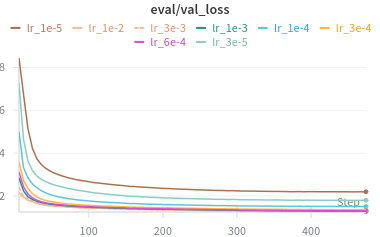
\includegraphics[width=\linewidth]{charts/learning_rate_1}
			\caption{Validation loss}
		\end{subfigure}\hfill
		\begin{subfigure}{0.49\textwidth}
			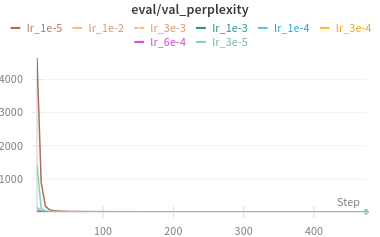
\includegraphics[width=\linewidth]{charts/learning_rate_0}
			\caption{Validation perplexity}
		\end{subfigure}
		\caption{Validation loss and perplexity across learning rate sweep (40K iterations, batch size 128).}
	\end{figure}

	\item[(b)] Increasing the learning rate progressively showed faster early loss reduction as we approached \texttt{1e-2}, indicating proximity to the stability boundary while still maintaining convergence. Pushing the rate far beyond this (e.g., \texttt{1e2}) produced highly erratic, non-convergent validation curves characteristic of divergence. Thus, the best-performing rate (\texttt{1e-2}) lies just below the edge of stability.

	\begin{figure}[H]
		\begin{subfigure}{0.49\textwidth}
			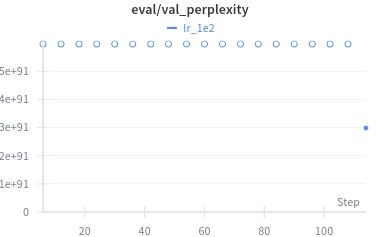
\includegraphics[width=\linewidth]{charts/learning_rate_edge_1}
			\caption{Validation loss}
		\end{subfigure}\hfill
		\begin{subfigure}{0.49\textwidth}
			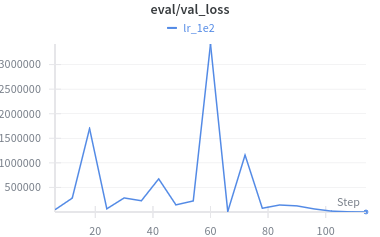
\includegraphics[width=\linewidth]{charts/learning_rate_edge_0}
			\caption{Validation perplexity}
		\end{subfigure}
		\caption{Validation loss and perplexity across learning rate sweep (40K iterations, batch size 128).}
	\end{figure}

\end{itemize}

\textit{Implemented in  \href{https://github.com/echung32/ece405-assignment1-basics/blob/main/slurm/train_learning_rate_sweep.slurm}{slurm/train\_learning\_rate\_sweep.slurm}}

\subsection{Problem (batch\_size\_experiment): Batch size variations (1 point)}

All batch-size runs used max LR \texttt{3e-3}, cosine decay with 2,000-iteration warmup, and
were trained for 10,000 iterations on TinyStories.

\begin{center}
\begin{tabular}{lrrr}
\hline
\textbf{Batch size} & \textbf{Final Val Loss} & \textbf{Final Val PPL} & \textbf{Wall-clock Time} \\
\hline
1   & 3.3106 & 27.40 & 3m 6s \\
8   & 2.4593 & 11.70 & 3m 11s \\
32  & 1.5403 &  4.67 & 7m 18s \\
64  & 1.4293 &  4.18 & 12m 23s \\
128 & 1.3563 &  3.88 & 22m 24s \\
256 & 1.3044 &  3.69 & 43m 38s \\
\hline
\end{tabular}
\end{center}

Batch sizes from 1 to 256 were evaluated for 10K steps (max LR \texttt{3e-3}, 2,000-step cosine warmup), showing steadily improved validation loss as batch size increased due to reduced gradient variance, with performance improving from 3.31 (batch 1) to 1.30 (batch 256). Although 128 and 256 achieved slightly better losses, batch size 64 was selected for future runs because it offered a strong trade-off between performance and efficiency (1.43 val loss in 12 minutes) compared to the marginal improvement at batch 256 (1.30 val loss in 43 minutes).

\begin{figure}[H]
	\begin{subfigure}{0.49\textwidth}
		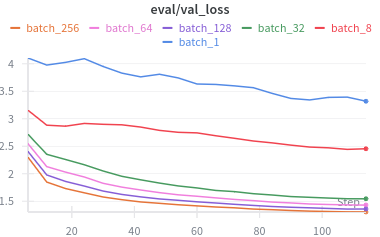
\includegraphics[width=\linewidth]{charts/batch_1}
		\caption{Validation loss}
	\end{subfigure}\hfill
	\begin{subfigure}{0.49\textwidth}
		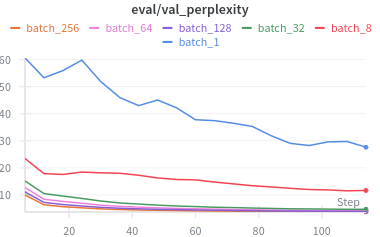
\includegraphics[width=\linewidth]{charts/batch_3}
		\caption{Validation perplexity}
	\end{subfigure}
	\caption{Validation loss and perplexity across batch sizes (10K iterations, max LR \texttt{3e-3}).}
\end{figure}

\textit{Implemented in  \href{https://github.com/echung32/ece405-assignment1-basics/blob/main/slurm/train_batch_sweep.slurm}{slurm/train\_batch\_sweep.slurm}}

\subsection{Problem (generate): Generate text (1 point)}

All the text generated below uses the checkpoint files for batch size 64, learning rate 3e-3.

\begin{modeloutput}{}
Once upon a time, there was a little boy named Tim. Tim was very happy and loved to play with his toys. One day, Tim found a big box of clothes in his room. He put them on and went to play with his friends.
Tim saw his friend, Sam, and asked, "What are you doing?" Sam replied, "I am playing with this clothes, but I have to separate them. I want to play with my toys." Tim thought for a moment and said, "I recommend we play a game with my toys."
Tim and Sam played a game of tag. They ran around the room, chasing each other and laughing. They had so much fun playing together. The sun started to set, and it was time for Sam to go home.
Tim and Sam said goodbye and promised to play together again soon. Tim went to bed, excited to play with his friends again tomorrow. And they all knew they would have more fun days together.<|endoftext|>
\end{modeloutput}
\noindent\textit{\small dataset=TinyStories, temp=0.8, top-p=0.9, prompt="Once upon a time,"}

\begin{modeloutput}{}
The equation 3x12 evaluates to the world. The sleepy little girl was filled with joy and excitement. She was filled with joy and joy. She knew that the sleepy little girl had worked so hard and she wanted to explore more.
The little girl packed her things and headed off. On the way, she came across a bright blue river. It was beautiful and the little girl loved it. She jumped in and swam around the river, exploring and enjoying the beautiful beauty.
The end.<|endoftext|>
\end{modeloutput}
\noindent\textit{\small dataset=TinyStories, temp=0.8, top-p=0.9, prompt="The equation 3x12 evaluates to"}

We can see that the fluency of the text is highly dependent on what the dataset was trained on; using anything other than storytelling terms on will likely not result in a coherent response, but using "Once upon a time," is more likely to produce a coherent response that makes some sense. In the case of "The equation 3x12 evaluates to", the model has no understanding of arithmetic and immediately drifts back to storytelling with no relation to the start.

As an exercise, the prompt was also evaluated at double the temperature (temp 1.6), which resulted in the following output:

\begin{modeloutput}{}
Once upon a time, an Jenny wanted to help it get mole apples. They filledions everySara read flap of expectingy logs until there would step Oneundayleum parade everyday. thoughts answered up intrigued all the moral of the compared names of itsurt whole novel from one car landscapes and Alice found an enormous green rotten deliver outside car O gun broke on rainy d clips sandwiches instead of apples crayon Fightingmyence today." From ine Please Mama, Mama ideas Bobo often Why wouldery Mia who would pack Bearnnved buying all was healthy pupils's favorite color sandcastle fl cob Joke enjoy as love yourself. Daisy have tested the3 guests play in gorOw chefs,erg Cats in enthusiastic hall trouble twice, twelveged shortsetings, pretending animalsPete spaceshiphing quarrel posesMrs wellrough Sunny being kind. Anna kept sear temperature promises Grandma showed her how patience wool always faaud ears exclaimed to taps blossouushed fair, and mayri Turtle Near nights shares funny piano inviting Sam. Sally understood what thick peace sounded like when all by beadsPenny with medals by her smooth dress focus.
From this experience, Anna gazed out for anReadyDon lighting the positiveimLuna opera attitudeivermered tall. Withwards everybody helping Tylerbers permissionhe seen hugging drippingAnn inBetty's scent, making
\end{modeloutput}
\noindent\textit{\small dataset=TinyStories, temp=1.6, top-p=0.9, prompt="Once upon a time,"}

It can be seen that doubling the temperature dramatically degrades output quality: the model produces incoherent word salad with broken grammar and invented tokens. High temperature flattens the probability distribution over the vocabulary, making low-probability tokens nearly as likely to be sampled as high-probability ones, which compounds across each generation step into nonsensical text.

\textit{Implemented in  \href{https://github.com/echung32/ece405-assignment1-basics/blob/main/cs336_basics/generation.py}{cs336\_basics/generation.py}}

\section{Ablations}

All ablation variants were trained for 10,000 iterations with batch size 64, cosine decay
schedule, and 2,000-iteration warmup, which matches the batch sweep baseline.

\subsection{Problem (layer\_norm\_ablation): Remove RMSNorm and train (1 point)}

\begin{center}
\begin{tabular}{llrrr}
\hline
\textbf{Variant} & \textbf{Max LR} & \textbf{Final Val Loss} & \textbf{Final Val PPL} & \textbf{Time} \\
\hline
Pre-norm (baseline) & \texttt{3e-3} & 1.4293 & 4.18 & 22m 24s \\
No norm (diverged) & \texttt{3e-3} & NaN & --- & 11m 38s \\
No norm (retry)    & \texttt{1e-5} & 3.0166 & 20.42 & 13m 23s \\
\hline
\end{tabular}
\end{center}

\begin{figure}[H]
	\begin{subfigure}{0.49\textwidth}
		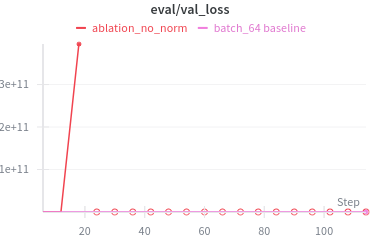
\includegraphics[width=\linewidth]{charts/layer_norm_ablation_1}
		\caption{Validation loss}
	\end{subfigure}\hfill
	\begin{subfigure}{0.49\textwidth}
		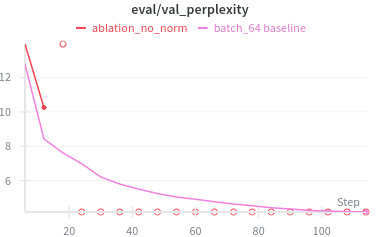
\includegraphics[width=\linewidth]{charts/layer_norm_ablation_3}
		\caption{Validation perplexity}
	\end{subfigure}
	\caption{Validation loss and perplexity for the no-norm ablation at \texttt{3e-3} learning rate.
	The pre-norm baseline is not visible in the loss plot as the no-norm run diverges and explodes.}
\end{figure}

\begin{figure}[H]
	\begin{subfigure}{0.49\textwidth}
		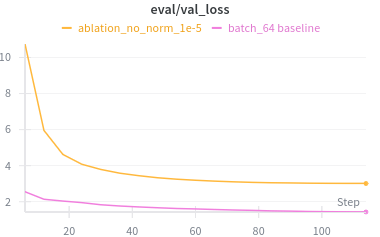
\includegraphics[width=\linewidth]{charts/layer_norm_ablation_1e5_1}
		\caption{Validation loss}
	\end{subfigure}\hfill
	\begin{subfigure}{0.49\textwidth}
		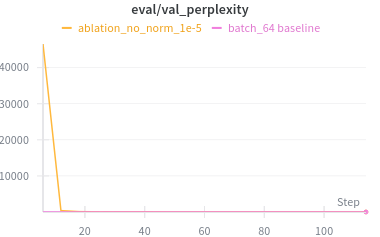
\includegraphics[width=\linewidth]{charts/layer_norm_ablation_1e5_0}
		\caption{Validation perplexity}
	\end{subfigure}
	\caption{Validation loss and perplexity for the no-norm ablation at \texttt{1e-5} learning rate,
	which does not explode but converges much more slowly than the pre-norm baseline.}
\end{figure}

Without RMSNorm, training at the optimal learning rate (\texttt{3e-3}) diverges rapidly. The loss spiked to $2.85 \times 10^{8}$ at iteration 1500 and became \texttt{NaN} by iteration 1600, with all subsequent evaluations producing \texttt{NaN}. Retrying with a drastically reduced learning rate (\texttt{1e-5}) prevented the explosion, but the model converged to a
much worse final validation loss of 3.0166 (ppl 20.42), compared to 1.4293 (ppl 4.18) for the pre-norm baseline.

\textit{Implemented in  \href{https://github.com/echung32/ece405-assignment1-basics/tree/main/cs336_basics/ablation}{cs336\_basics/ablation}}

\subsection{Problem (pre\_norm\_ablation): Implement post-norm and train (1 point)}

\begin{center}
\begin{tabular}{lrrr}
\hline
\textbf{Variant} & \textbf{Final Val Loss} & \textbf{Final Val PPL} & \textbf{Time} \\
\hline
Pre-norm (baseline) & 1.4293 & 4.18 & 22m 24s \\
Post-norm           & 1.4716 & 4.36 & 12m 2s \\
\hline
\end{tabular}
\end{center}

\begin{figure}[H]
	\begin{subfigure}{0.49\textwidth}
		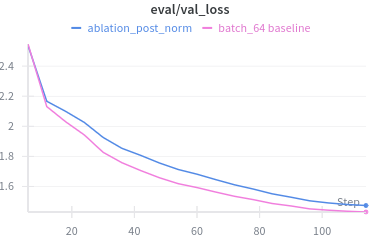
\includegraphics[width=\linewidth]{charts/postnorm_ablation_1}
		\caption{Validation loss}
	\end{subfigure}\hfill
	\begin{subfigure}{0.49\textwidth}
		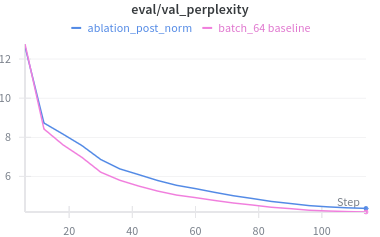
\includegraphics[width=\linewidth]{charts/postnorm_ablation_3}
		\caption{Validation perplexity}
	\end{subfigure}
	\caption{Validation loss and perplexity comparing pre-norm and post-norm variants (10K iterations, max LR \texttt{3e-3}).}
\end{figure}

\textit{Implemented in  \href{https://github.com/echung32/ece405-assignment1-basics/tree/main/cs336_basics/ablation}{cs336\_basics/ablation}}

\subsection{Problem (no\_pos\_emb): Implement NoPE (1 point)}

\begin{center}
\begin{tabular}{lrrr}
\hline
\textbf{Variant} & \textbf{Final Val Loss} & \textbf{Final Val PPL} & \textbf{Time} \\
\hline
RoPE (baseline) & 1.4293 & 4.18 & 22m 24s \\
NoPE            & 1.4981 & 4.47 & 11m 52s \\
\hline
\end{tabular}
\end{center}

\begin{figure}[H]
	\begin{subfigure}{0.49\textwidth}
		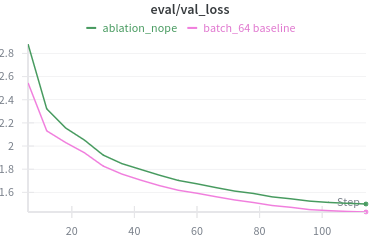
\includegraphics[width=\linewidth]{charts/no_pos_emb_ablation_1}
		\caption{Validation loss}
	\end{subfigure}\hfill
	\begin{subfigure}{0.49\textwidth}
		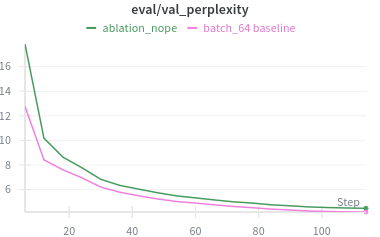
\includegraphics[width=\linewidth]{charts/no_pos_emb_ablation_3}
		\caption{Validation perplexity}
	\end{subfigure}
	\caption{Validation loss and perplexity comparing RoPE and NoPE variants (10K iterations, max LR \texttt{3e-3}).}
\end{figure}

\textit{Implemented in  \href{https://github.com/echung32/ece405-assignment1-basics/tree/main/cs336_basics/ablation}{cs336\_basics/ablation}}

\subsection{Problem (swiglu\_ablation): SwiGLU vs.\ SiLU (1 point)}

\begin{center}
\begin{tabular}{lrrr}
\hline
\textbf{Variant} & \textbf{Final Val Loss} & \textbf{Final Val PPL} & \textbf{Time} \\
\hline
SwiGLU (baseline) & 1.4293 & 4.18 & 22m 24s \\
SiLU              & 1.4466 & 4.25 & 11m 52s \\
\hline
\end{tabular}
\end{center}

The SiLU model achieves a final val loss of 1.4466 (ppl 4.25), only 1.2\% worse than the SwiGLU baseline. Both converged smoothly at \texttt{3e-3}. The minimal difference suggests that at this model scale (22.7M SwiGLU vs. 22.8M SiLU parameters, 10K iterations, TinyStories), the gating mechanism of SwiGLU provides only a marginal benefit over a simpler SiLU activation.

\begin{figure}[H]
	\begin{subfigure}{0.49\textwidth}
		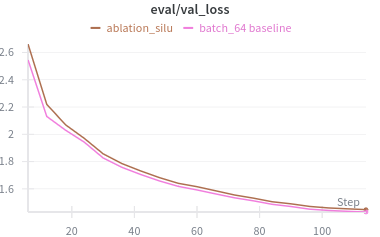
\includegraphics[width=\linewidth]{charts/silu_ablation_1}
		\caption{Validation loss}
	\end{subfigure}\hfill
	\begin{subfigure}{0.49\textwidth}
		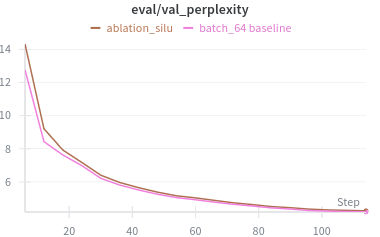
\includegraphics[width=\linewidth]{charts/silu_ablation_3}
		\caption{Validation perplexity}
	\end{subfigure}
	\caption{Validation loss and perplexity comparing SwiGLU and SiLU variants (10K iterations, max LR \texttt{3e-3}).}
\end{figure}

\textit{Implemented in  \href{https://github.com/echung32/ece405-assignment1-basics/tree/main/cs336_basics/ablation}{cs336\_basics/ablation}}

\subsection{Problem (main\_experiment): Experiment on OWT (2 points)}

\begin{figure}[H]
	\begin{subfigure}{0.49\textwidth}
		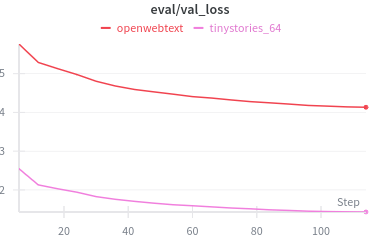
\includegraphics[width=\linewidth]{charts/openwebtext_0}
		\caption{Validation loss}
	\end{subfigure}\hfill
	\begin{subfigure}{0.49\textwidth}
		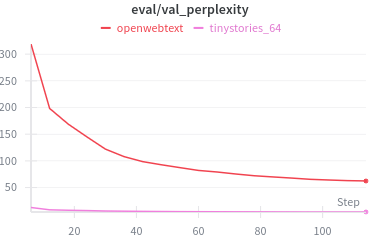
\includegraphics[width=\linewidth]{charts/openwebtext_1}
		\caption{Validation perplexity}
	\end{subfigure}
	\caption{Validation loss and perplexity for OWT vs.\ TinyStories baseline (10K iterations, max LR \texttt{3e-3}, batch size 64).}
\end{figure}

After 10K iterations, the OpenWebText (OWT) model has much higher validation loss and perplexity than TinyStories, and the gap remains roughly constant throughout training, indicating OWT is far from converged under the same computational budget. The generated OWT samples are stylistically web-like but semantically incoherent, with repetitive and hollow phrasing (e.g., “the function of the function”). Despite identical architecture and training steps, the model must spread its limited capacity across many domains and has not trained long enough to capture OWT’s broader distribution.

\begin{modeloutput}{}
Once upon a time, we have to say that we have the upper hand that we are going to have to wait for.

I believe that we will have to ask ourselves to give a more accurate description, even if they're not saying that we are, in fact, just the right people to express that opinion, but we have to give the impression that we have a way to know that we will be out of touch.

"We will also like to look at what we will say to you," I said.

I didn't think we would have a great time to do the same. But they had to do a lot of things, for the majority of the time, not to do it. I'm not worried that we will get more intelligence.

I think this is a good time to do this. But for a while, I think that's enough to say the least.

But the fact is, it seems like every day.

So, I feel like the fact that we know the United States are in good shape. I think they have a really good understanding of what we're doing.

We know the United States is too often in the realm of certainty, and I think that's just as much more appropriate. We know
\end{modeloutput}
\noindent\textit{\small dataset=OpenWebText, temp=0.8, top-p=0.9, prompt="Once upon a time,"}

\begin{modeloutput}{}
The equation 3x12 evaluates to any extent the difference between "approach" and "due-value".

Note that there is a sense of fact that the function of the function is the same as the function to be defined by the function and the function. For example, if the function is a function to have the function, which should be "likely" and "to have the function that you can find".

The function of the function of the function is called when the function takes a function. In that case, it is called function which functions it. For example, the function is called "over" or "in" -- which is the function of the function (1) and the function (2) is called "in".

The function can be used to define a function and returns the function of the function.

When the function takes a function, it doesn't matter.

The function should function as a function for the function.

The function takes a function that calls it's function. It needs the function to do that, which is why it does.

It is crucial for the function to execute this function.

It is important to note that it is important to keep this function in place.

It is
\end{modeloutput}
\noindent\textit{\small dataset=OpenWebText, temp=0.8, top-p=0.9, prompt="The equation 3x12 evaluates to"}

\textit{Implemented in  \href{https://github.com/echung32/ece405-assignment1-basics/blob/main/cs336_basics/generation.py}{cs336\_basics/generation.py}}

\appendix

\section{Appendix}

\subsection{Code Availability}

All code mentioned in this report is available at \href{https://github.com/echung32/ece405-assignment1-basics}{github.com/echung32/ece405-assignment1-basics}

\subsection{Training Logs}

All training logs and ablation studies are available at Weights \& Biases:

\begin{itemize}
	\item TinyStories learning rate sweep: \href{https://wandb.ai/echung32-ece405/ece405-tinystories-lrsweep}{wandb.ai/echung32-ece405/ece405-tinystories-lrsweep}
	\item TinyStories batch sweep: \href{https://wandb.ai/echung32-ece405/ece405-tinystories-batchsweep}{wandb.ai/echung32-ece405/ece405-tinystories-batchsweep}
	\item TinyStories ablation studies: \href{https://wandb.ai/echung32-ece405/ece405-tinystories-ablation}{wandb.ai/echung32-ece405/ece405-tinystories-ablation}
	\item OpenWebText: \href{https://wandb.ai/echung32-ece405/ece405-openwebtext}{wandb.ai/echung32-ece405/ece405-openwebtext}
\end{itemize}

\end{document}
